\section{Lokalizacja twarzy na obrazie}
\label{sec:face-detect}
W ciągu ostatnich lat obserwuje się bardzo dynamiczny rozwój biometrii.
Aplikacje analizujące biometryczne cechy użytkowników znalazły swoje
zastosowanie między innymi w systemach zabezpieczeń i monitoringu, robotyce,
komputerach przenośnych, aparatach i kamerach cyfrowych czy nawet w nowoczesnych
telefonach komórkowych. Pośród szeregu cech które mogą zostać poddane analizie,
szczególnym zainteresowaniem cieszy się analiza ludzkiej twarzy. Systemy
posiadające możliwość zlokalizowania na obrazie twarzy od pewnego czasu
towarzyszą nam w życiu codziennym. Niemniej jednak większość istniejących
algorytmów pozwalających na rozwiązanie tego problemu jest
dosyć skomplikowana i~ma~bardzo konkretne wymagania zarówno co do platformy sprzętowej
jak i~jakości obrazu który będzie poddawany analizie. Dlatego też stworzenie
implementacji dla platformy o~bardzo ograniczonych zasobach obliczeniowych i
pamięciowych jest dużym wyzwaniem. Celem niniejszego rozdziału jest
przedstawienie podstawowych rodzajów algorytmów lokalizacji twarzy oraz
wskazanie ich wad i zalet. W dalszej części znajduje się szczegółowy opis
stworzonej implementacji algorytmu zastosowanego w realizowanej pracy magisterskiej.

\subsection{Algorytmy}
W ciągu ostatnich kliku lat rozwijanych było wiele różnych podejść poprawiających
wydajność procesu lokalizacji ludzkiej twarzy. Wśród nich można wyróżnić klika
głównych kategorii. Pierwszą z nich jest metoda opierająca się o bazę wiedzy.
Metoda ta pozwala na odszukiwanie niezmiennych cech twarzy nawet w bardzo
skomplikowanym otoczeniu, a przez to pozwala na ustalenie pozycji twarzy. Tego
typu podejście do problemu eliminuje problemy z uwzględnianiem ułożenia i pozycji
twarzy na obrazie. Statystyczny opis zależności pomiędzy poszczególnymi cechami
twarzy pozwala na stworzenie modelu który może posłużyć do zbudowania szablonu
twarzy dzięki któremu będziemy w stanie jednoznacznie stwierdzić czy na obrazie
widoczna jest twarz czy nie. Z takiego ujęcia problemu wywodzi się kolejna metoda
nazywana metodą porównywaniu szablonów (ang. template matching). Do stworzenia
wspomnianego szablonu twarzy mogą posłużyć takie parametry jak na przykład kolor
skóry, faktura twarzy czy też budowa twarzy. Wśród metod bazujących na
porównywaniu szablonów można wyróżnić dwa podejścia. Pierwsze z~nich oparte jest
bezpośrednio na opisie cech twarzy i korzysta z opisu zależności pomiędzy
parametrami twarzy jako szablonu, odszukując najbardziej pasujący do szablonu
fragment obrazu. Drugim podejściem jest stosowanie globalnego szablonu bazującego
na metrykach będących sumą poszczególnych cech za pomocą których jest opisany
szablon. Pierwsze podejście wymaga obrazu o stosunkowo dużej rozdzielczości ale
ponieważ nie bazuje ono na wszystkich punktach obrazu będzie obliczeniowo
bardziej wydajne niż podejście oparte o szablon globalny które może wymagać
przeszukania potencjalnie dużo większej grupy punktów obrazu wejściowego. Główną
wadą przestawionych do tej pory rozwiązań są ich dosyć wysokie wymagania.
Każdy z omówionych do tej pory algorytmów wymagał wykonywania kosztownych
obliczeń mających na celu, poprzez dokonywanie przekształceń, dopasowanie modelu
szablonu do zawartości obrazu wejściowego. Tak więc wykorzystanie tego typu
algorytmów wiąże się z koniecznością użycia stosunkowo mocnych jednostek
obliczeniowych, co w przypadku platformy embeded mogłoby być problematyczne.

Zupełnie innym podejściem do problemu lokalizacji twarzy jest wykorzystywanie
koloru skóry do odszukania fragmentów obrazu które potencjalnie mogłyby zwierać
twarz. Rozwiązania oparte o analizę kolorów można podzielić na dwie grupy. W
pierwszej znajdują się rozwiązania bazujące na jednolitym kolorze tła, w drugiej
natomiast obraz wejściowy może zawierać tło o dowolnym stopniu złożoności.
Pierwsza z przedstawionych grup w znakomity sposób upraszcza problem odnalezienia
twarzy gdyż często usunięcie koloru tła z obrazu gwarantuje nam odnalezienie
wszystkich twarzy, zakładając, że obraz zawiera jedynie twarze. Jednakże jest to
podejście nakładające duże ograniczenia na warunki w jakich odbywa się akwizycja
obrazu. Dlatego też znacznie częściej porusza się problem lokalizacji twarzy w
oparciu o analizę kolorów, z użyciem obrazów zawierających niejednokrotnie tło o
bardzo wysokim stopniu złożoności. Niemniej jednak wszystkie rozwiązania bazujące
jedynie na segmentacji kolorów są w bardzo wysokim stopniu zależne od warunków w
jakim pobierany jest obraz wejściowy. Ze względu na zmieniające się warunki
otocznia może okazać się, że nasz algorytm nie uwzględnia wszystkich kolorów
skóry. Dodatkowym utrudnieniem jest pojawianie się grup pikseli które zostały
zakwalifikowane jako kolor skóry pomimo, że z twarzą nie mają nic wspólnego.
Problem ten jest szczególnie uciążliwy w przypadku obrazów o małych rozmiarach,
gdyż trudno jest wtedy odróżnić twarz od szumów powstałych wskutek warunków
otocznia, w których obraz był pobierany. Pomimo licznych swoich licznych wad
segmentacja kolorów jest jedną z najszybszych metod klasyfikacji obrazów pod
kątem obecności twarzy na obrazie. Co więcej narzut obliczeniowy na zastosowanie
klasyfikatora bazującego o model kolorów skóry jest proporcjonalny do rozmiarów
pobranego obrazu. Niestety jak się okazuje w praktyce sama segmentacja kolorów
jest niewystarczająca i wymaga
użycia dodatkowych metod w celu potwierdzenia odnalezienia twarzy.

Kolejnym ciekawym rozwiązaniem pozwalającym na odszukanie twarzy na ruchomym
obrazie jest analiza ruchów twarzy. W tego typu rozwiązaniach obecność twarzy
w~sekwencji wideo wykrywana jest na podstawie detekcji ruchów charakterystycznych
dla ludzkiej twarzy, takich jak na przykład ruchy powiek. Mruganie jest ruchem na
tyle specyficznym, że wykrycie go pozwala jednoznacznie wnioskować o lokalizacji
twarzy na obrazie. Niestety przetwarzanie kilkudziesięciu klatek na sekundę o
rozmiarach pozwalających na zarejestrowanie ruchu powiek stawia dosyć wygórowane
wymagania związane nie tylko z algorytmem ale również z ilością danych jakie
klasyfikator musi przetworzyć w ciągu każdej sekundy nagrania. Istnieje jeszcze
wiele innych rozwiązań bazujących na bardzo wyszukanych metodach, jak na przykład
użycie sieci neuronowych, jednakże ze względu na ich wygórowane wymagania,
wykorzystanie jednego z nich dla platformy embeded z ograniczonymi zasobami
obliczeniowymi i pamięciowymi jest niezwykle trudne, a w niektórych przypadkach
niemal całkowicie niemożliwe.

Algorytm implementowany w ramach pracy magisterskiej bazuje na podejściu opartym
o segmentację kolorów. Aby wyeliminować niedoskonałości płynące z tego podejścia
algorytm w ostatnie fazie wykorzystuje informację o najprostszych cechach twarzy
w celu potwierdzenia obecności twarzy w obszarach zaklasyfikowanych jako kolor
skóry. Zastosowanie tego typu połączenia dwóch technik zaowocowało postaniem
algorytmu nie tylko szybkiego ale zarazem dającego stosunkowo dobre wyniki
analizy.

\subsection{Implementacja}
Implementacja modułu do lokalizacji twarzy na obrazie pobranym z kamery robota
została w całości oparta o algorytm zaproponowany w artykule zatytułowanym 'Simple Face-detection Algorithm Based on Minimum
Facial Features' \cite{SimpleFaceDetectionAlgorithm}. Autorzy do rozwiązania
problemu używają obrazów o małej rozdzielczości opisanych za pomocą modelu
kolorów RGB\footnote{RGB (z ang. Red Green Blue) - popularny w grafice model
przestrzeni barw}.

Zgodnie ze wskazówkami znalezionymi we wspomnianej publikacji, pierwszym krokiem
na drodze do zlokalizowania twarzy na obrazie jest akwizycja danych z kamery.
Przesłany z kamery obraz automatycznie jest poddawany podstawowej korekcji
mającej na celu dopasowanie balansu bieli oraz  dopasowanie ostrości. Tak
przygotowany obraz poddawany jest binaryzacji. Celem wspomnianego procesu jest
odnalezienie na obrazie obszarów będących w kolorze skóry oraz włosów. Zanim
jednak detekcja interesujących nas obszarów będzie możliwa, konieczne jest
przeprowadzenie normalizacji modelu RGB. Zabieg tego typu pozwoli na usunięcie
zakłóceń wywołanych przez światła i cienie na obrazie pobranym z kamery robota.

Opisany proces normalizacji przeprowadzany jest poprzez pobranie wartości
poszczególnych kanałów RGB danego piksela obrazu, a następnie podzielenie tak
otrzymanej liczby przez sumę wartości wszystkich kanałów danego punktu.
Korzystając z takiego przepisu otrzymujemy zestaw równań \ref{eq:rgb-norm-r},
\ref{eq:rgb-norm-g}, \ref{eq:rgb-norm-b} opisujący normalizację każdego kanału z
palety RGB.

\begin{eqnarray}
\label{eq:rgb-norm-r}
r = \frac{R}{R + G +B}\\
\label{eq:rgb-norm-g}
g = \frac{G}{R + G +B}\\
\label{eq:rgb-norm-b}
b = \frac{B}{R + G +B}
\end{eqnarray} 

Na tak przygotowanym obrazie można już podjąć próbę odszukania punktów w~kolorze
skóry i włosów. Do tego celu użyte zostały równania zaproponowane przez autorów
pracy źródłowej. Określają one rozkład kolorów ludzkiej skóry i włosów
wyznaczonych, jak twierdzą autorzy, w sposób eksperymentalny. Bazując na takich
założeniach ustalony został górny $F_1(r)$ i dolny $F_2(r)$ zakres kolorów w
jakich może znaleźć się ludzka skóra (rów. \ref{eq:f1-r}, \ref{eq:f2-r}).
\begin{eqnarray}
\label{eq:f1-r}
F_1\left(r\right) = -1.376r^2 + 1.0743r + 0.2\\
\label{eq:f2-r}
F_2\left(r\right) = -0.776r^2 + 0.5601r + 0.18
\end{eqnarray}
Należy jednak zauważyć, że w zdefiniowanych w ten sposób równaniach mieści się
również kolor biały $r = g = 0.33$ dlatego też należy dodać następujący
warunek (rów. \ref{eq:white-rm}) usuwający niechciany kolor z obszaru
zainteresowania.
\begin{equation}
\label{eq:white-rm}
w = \left(r - 0.33\right)^2 + \left(g - 0.33\right)^2 > 0.001
\end{equation}
Po połączeniu obydwu równań otrzymujemy następujący układ równań opisujący
zakres kolorów jakie powinny reprezentować ludzką skórę. 
\begin{equation}
S = \left\{ 
\begin{array}{l l}
  1 & \quad \mbox{dla $g < F_1\left(r\right) \cap g > F_2\left(r\right) \cap w
  > 0.001$}\\ 0 & \quad \mbox{dla pozostałych}\\ \end{array} \right. 
  \label{skinEq1}
\end{equation}
Praktyczne doświadczenia z wykrywaniem obszarów skóry z zastosowaniem równania
\ref{skinEq1} wykazały iż niemal wszystkie obszary o kolorze skóry zostały
prawidłowo zaklasyfikowane. Znakomita większość pikseli nie stanowiących koloru
skóry została zastąpiona kolorem czarnym. Niemniej jednak wiele pikseli o
kolorze niebieskim, żółtym i szarym również została błędnie sklasyfikowana. 

Aby wyeliminować tego rodzaju efekt należy wykorzystać kryteria klasyfikacji oparte
o przestrzeń kolorów HSI \footnote{HSI (z ang. Hue Saturation Intensity) -
model przestrzeni bar nawiązujący do sposobu w jaki widzi ludzki narząd wzroku }.
W równaniu \ref{eq:rgb2hsi} przedstawiono zależność pomiędzy modelem RGB a HSI.
\begin{equation}
\label{eq:rgb2hsi}
\begin{array}{l}
\phi = cos^{-1}\left\{ \frac{0.5[(R-G)+(R-B)]}{\sqrt{(R-G)^2 + (R-B)(G-B)}}
\right\}\\\\
\left\{
\begin{array}{l l}
H=\phi & \mbox{dla B }\leq G\\
H=360^{\circ}-\phi & \mbox{dla B} > G
\end{array}
\right.
\end{array}
\end{equation}
Po skorzystaniu z przestrzeni HSI otrzymujemy następujący przepis  (rów.
\ref{eq:hsi-skin-color}) na kolor skóry.
\begin{equation}
\label{eq:hsi-skin-color}
S = \left\{ 
\begin{array}{l l}
  1 & \quad \mbox{dla $g < F_1\left(r\right) \cap g > F_2\left(r\right) \cap w
  > 0.001 \cap (H > 240 \cup H \leq 20 )$}\\ 0 & \quad \mbox{dla pozostałych}\\
  \end{array} \right.
  \label{skinEq2}
\end{equation}
Przy tak zdefiniowanym klasyfikatorze dokonywana jest binaryzacja całego obrazu.
Po~przeprowadzeniu binaryzacji przeprowadzana jest kwantyzacja obrazu za pomocą
próbki o rozmiarze i wysokości pięciu pikseli. Pozwala to zmniejszyć
rozdzielczość obrazu, a~co~za~tym idzie wyeliminować pewne rodzaje szumu oraz
znacznie uprościć dalsze obliczenia. Wspomniany proces kwantyzacji polega na
przeliczeniu liczby pikseli w kolorze skóry i~kolorze czarnym w ramach 25
pikseli pobranych jako próbka obrazu. A następnie na podstawie wartości progowej
podjęcie decyzji czy cała próbka zostanie oznaczona kolorem skóry czy kolorem
czarnym. W ramach implementacji wartość progu została ustalona na poziomie 12
pikseli, oznacza to, że wszystkie próbki zawierające więcej niż 12 pikseli
czarnych są w całości oznaczane jako obszar niezawierający skóry i na odwrót.

Metodą weryfikacji pozwalającą stwierdzić czy znaleziony obszar
jest elementem twarzy polega na odnalezieniu w sąsiedztwie obszarów będących w
kolorze włosów. Jest to prymitywna metoda nie gwarantująca 100\% poprawności,
ale na potrzeby tej pracy magisterskiej jest w zupełności wystarczająca. 

Do wykrywania potencjalnych obszarów w którym znajdują się włosy wykorzystywana
jest składowa intensywności modelu HSI. Zależność pomiędzy składowymi modelu RGB
a wspomnianą intensywnością opisana jest za pomocą równania
\ref{eq:rgb-intensity-hsi}
\begin{equation}
	\label{eq:rgb-intensity-hsi}
	I = \frac{1}{3}\left(R+G+B\right)
\end{equation}

Tak zdefiniowany komponent intensywności może zostać wykorzystany do ewaluacji
jasności obrazka, a co za tym idzie może posłużyć do odnalezienia ciemnych
obszarów które mogą stanowić obszar włosów. W oparciu o dane eksperymentalne
zostało zdefiniowane następujące równanie opisujące zakres
kolorów w którym mogących stanowić włosy. 
\begin{equation}
\label{eq:hair-bin}
H = \left\{ 
\begin{array}{l l}
  1 & \quad \mbox{dla $\left( I < 80 \cap \left(B - G < 15 \cup B - R < 15
  \right) \right) \cup  \left( 20 < H \leq 40 \right) $} \\ 0 & \quad
  \mbox{dla pozostałych}\\ \end{array} \right.
\end{equation}

Po przeprowadzeniu binaryzacji za pomocą równania \ref{eq:hair-bin},  podobnie
jak to miało miejsce w przypadku detekcji skóry, przeprowadzana jest kwantyzacja
otrzymanego obrazu. Następnym krokiem algorytmu jest wyszukanie wszystkich
obszarów które zostały zaklasyfikowane jako kolor skóry i odnalezienie
korespondującego z nimi obszaru włosów. Dla każdego obszaru wyznaczany jest
minimalny prostokąt otaczający, a następnie sprawdzany jest w jakiej relacji
jest on z pozostałymi elementami. W przypadku gdy obszar reprezentujący skórę oraz
włosy znajdą się w jednej z dozwolonych konfiguracji (rys.
\ref{fig:supported-relations}) obszar jest klasyfikowany jako twarz. 

\begin{figure}[ht!]
 \centering
 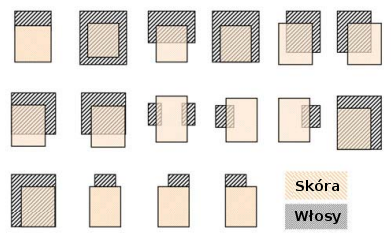
\includegraphics[width=\textwidth]{../images/ch04/bounding-boxes.png}
 \caption{Dopuszczalne relacje pomiędzy wykrytymi obszarami skóry i włosów
 (źródło: \cite{SimpleFaceDetectionAlgorithm})}
 \label{fig:supported-relations}
\end{figure}

\subsection{Wnioski i podsumowanie}
Opisana implementacja poddawana była licznym testom mających na celu wyznaczenie
skuteczności z jaką algorytm lokalizuje twarz na zdjęciach różnych osób w
różnych warunkach oświetleniowych. Już pierwsze testy wykazały, że gdy akwizycja
obrazu odbywa się w warunkach laboratoryjnych algorytm bez problemów znajduje
twarze na zdefiniowanym obrazie (rys. \ref{fig:face-detect-result}).
\begin{figure}[ht!]
 \centering
 \subfloat[Obraz początkowy]{\label{fig:fd1}
 	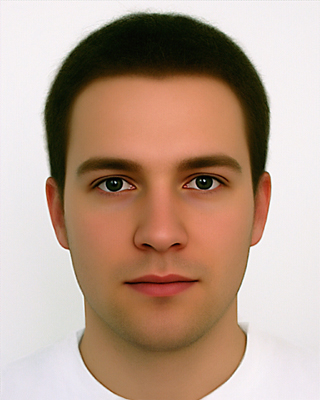
\includegraphics[width=0.32\textwidth]{../images/ch03/start.jpg}}
 	\subfloat[Obraz po binaryzacji]{\label{fig:fd2}
 	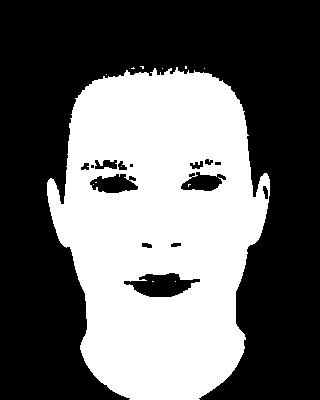
\includegraphics[width=0.32\textwidth]{../images/ch03/step2.jpg}}
 \subfloat[Wykryta twarz]{\label{fig:f3}
 	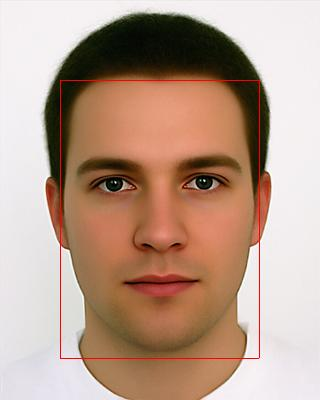
\includegraphics[width=0.32\textwidth]{../images/ch03/final.jpg}}
 \caption[caption-fdetect]{Weryfikacja działaniu algorytmu dla zdjęcia
 wykonanego w warunkach laboratoryjnych \footnotemark}
 \label{fig:face-detect-result}
\end{figure}
\footnotetext{źródło obrazu początkowego: Beauty Check - \url{http://www.uni-regensburg.de/}}

Niestety w przypadku gdy zdjęcie zostało wykonane w złych warunkach
oświetleniowych lub w tle znajdują się elementy w drewniane lub czarne algorytm
nie sprawdza się i z bardzo małą skutecznością lokalizuje twarz. Źródłem takiego
stanu rzeczy jest oparcie działania całego algorytmu o analizę kolorów. W
celu osiągnięcia większej skuteczność w działaniu algorytmu konieczne byłoby
wykorzystanie metod bazujących nie tylko na kolorach ale również na geometrii
twarzy. Aby to stało się możliwe konieczne jest zwiększenie dostępnej ilości
pamięci ponieważ w obecnej konfiguracji jest ona nie wystarczająca. Należałoby
rozważyć również wykorzystanie szybszego procesora gdyż niektóre metody bazujące
np. na porównywaniu szablonów wymagają przeprowadzania transformacji
geometrycznych na obrazie co przy wykorzystaniu obecnej jednostki obliczeniowej
może być niezwykle czasochłonne. 
Dzięki udoskonalonemu procesowi akwizycji danych z kamery możliwe jest
zrezygnowanie z analizowania obrazu na mikrokontrolerze i przeprowadzenie
profesjonalnej lokalizacji twarzy za pomocą komputera. Jedynym
ograniczeniem takiego podejścia jest przepustowość obecnego kanału
komunikacyjnego. 